\documentclass[notheorems,mathserif,table,compress]{beamer}  %dvipdfm选项是关键,否则编译统统通不过
%%------------------------常用宏包------------------------
%%注意, beamer 会默认使用下列宏包: amsthm, graphicx, hyperref, color, xcolor, 等等
\usepackage{fontspec,xunicode,xltxtra}  % for XeTeX
\usepackage{verbatim}
\usepackage{mathabx}
\usepackage{tcolorbox}
\usepackage{subfigure} %%图形或表格并排排列
\usepackage{colortbl,dcolumn}     %% 彩色表格
\usepackage{styles/zhfontcfg}
\usepackage{styles/iplouclistings}
\usepackage{styles/iplouccfg}
\usepackage{fancybox}     %% 定义zhushadow时用到
%%------------------------ThemeColorFont------------------------
\usetheme{Madrid}
\usecolortheme{whale}      % Outer color themes, 其他选择: whale, seahorse, dolphin . 换一个编译看看有什么不同.
\usecolortheme{orchid}     % Inner color themes, 其他选择: lily, orchid
\useinnertheme[shadow]{rounded}
\useoutertheme{miniframes} 
\usefonttheme{serif}
\setbeamertemplate{background canvas}[vertical shading][bottom=white,top=structure.fg!7] %%背景色, 上25%的蓝, 过渡到下白.
\setbeamertemplate{theorems}[numbered]
\setbeamertemplate{navigation symbols}{}   %% 去掉页面下方默认的导航条.

\newcommand\zhushadow[2][purple]{\hskip5pt\shadowbox{\color{#1}\small\kai #2\vspace{3mm}}}

%%------------------------LOGO------------------------
\pgfdeclareimage[height=1cm]{university-logo}{Git-Logo-2Color.png}
\logo{\pgfuseimage{university-logo}}
%%----------------------------------------------------

%%------------------------MISC------------------------
\graphicspath{{figures/}}         %% 图片路径. 本文的图片都放在这个文件夹里了.
%%------------------------正文------------------------
\begin{document}
\XeTeXlinebreaklocale "zh"         % 表示用中文的断行
\XeTeXlinebreakskip = 0pt plus 1pt % 多一点调整的空间
%%----------------------------------------------------------
%% This is only inserted into the PDF information catalog. Can be left
%% out.
%%%
%% Delete this, if you do not want the table of contents to pop up at
%% the beginning of each subsection:
\AtBeginSection[]{                              % 在每个Section前都会加入的Frame
  \frame<handout:0>{
    \frametitle{Contents}\small
    \tableofcontents[current,currentsubsection]
  }
}

\AtBeginSubsection[]                            % 在每个子段落之前
{
  \frame<handout:0>                             % handout:0 表示只在手稿中出现
  {
    \frametitle{Contents}\small
    \tableofcontents[current,currentsubsection] % 显示在目录中加亮的当前章节
  }
}

%%----------------------------------------------------------
\title{开源软件之————git学习篇}
\author[zhu]{主讲人~~~~~\textcolor{olive}{朱亚菲}\\
    \quad 幻灯片制作~~\textcolor{olive}{朱亚菲}}
\institute[中国海洋大学]{\small\textcolor{violet}{中国海洋大学~~信息科学与工程学院}}
\date{2014~年~9~月~19~日}
%\titlegraphic{\vspace{-6em}\includegraphics[height=7cm]{ouc}\vspace{-6em}}
\frame{ \titlepage }
%%----------------------------------------------------------


%%----------------------------------------------------------
\section{Git简介}

\subsection{Git是什么?}

\begin{frame}
  \zhushadow{Git} Git是目前世界上最先进的分布式版本控制系统!

  \zhushadow{版本控制} 
  \begin{figure}
    \begin{minipage}[t]{0.25\linewidth} 
    \leftline{
\includegraphics[width=\linewidth]{word.png}}
  \end{minipage}
  \hspace{1cm}
  \begin{minipage}[t]{0.1\linewidth} 
    \rowcolors[]{1}{blue!20}{blue!10}
  \resizebox{3\hsize}{!}{$\begin{tabular}{|c|c|c|c|c|}  
  \hline
  版本 & 用户  &        说明            &    日期       \\
  \hline
    1  & 张三  & 删除了实验室规则说明5   & 7/12 10:38   \\ 
  \hline
    2  & 李四  &     加入一幅图片       &  7/12 18:09   \\
  \hline
    3  & 张三  &   修改了README.md      &  7/13 9:51    \\
  \hline
    4  & 李四  &   新增一种绘图颜色      &  7/14 15:17   \\
  \hline 
  \end{tabular}$}
  \end{minipage}
  \end{figure}

  \zhushadow{集中式vs分布式} 
  \begin{figure}
  \vspace{-1mm}
  \begin{minipage}[t]{0.2\linewidth} 
    \centering 
    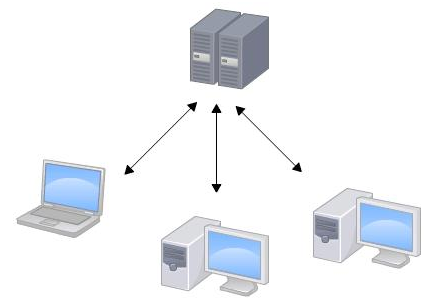
\includegraphics[width=\linewidth]{集中式.png} \\
    {\heiti\textcolor{blue}{集中式}}
  \end{minipage}
  \hspace{2cm}
  \begin{minipage}[t]{0.2\linewidth} 
    \centering 
    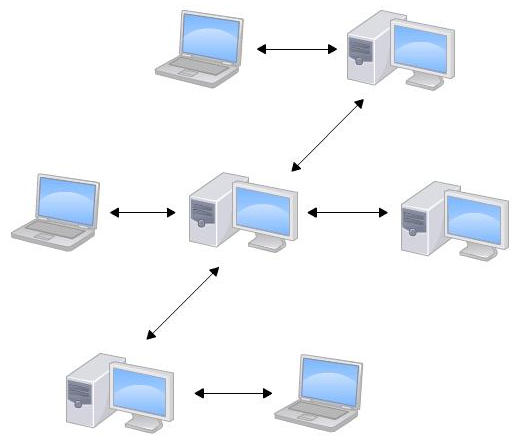
\includegraphics[width=\linewidth]{分布式.png} \\
    {\heiti\textcolor{blue}{分布式}}
  \end{minipage}
\\
\end{figure}
\end{frame}


\subsection{Git的诞生}

\begin{frame}
  同生活中的许多伟大事件一样,Git 诞生于一个极富纷争大举创新的年代。Linux 内核开源项目有着为数众广的参与者。绝大多数的 Linux 内核维护工作都花在了提交补丁和保存归档的繁琐事务上(1991-2002年间)。到 2002 年,整个项目组开始启用分布式版本控制系统   BitKeeper 来管理和维护代码。\\
  到了 2005 年,开发 BitKeeper 的商业公司同 Linux 内核开源社区的合作关系结束,他们收回了免费使用 BitKeeper 的权力。这就迫使 Linux 开源社区(特别是 Linux 的缔造者 Linus Torvalds )不得不吸取教训,只有开发一套属于自己的版本控制系统才不至于重蹈覆辙。
\end{frame}

\section{Git使用}

\begin{frame}
  \frametitle{Prearrange}
  \flushleft
  \begin{enumerate}
  \item 安装
  \item 设置
  \newline
  \begin{tabular}{|l|}
  \hline
  \$git config --global user.name ``Your Name" \\
  \$git config --global user.email ``email@example.com"\\
  \hline
  \end{tabular}
  \item 创建版本库
  \begin{figure}[h]
  %\centering
  \centerline{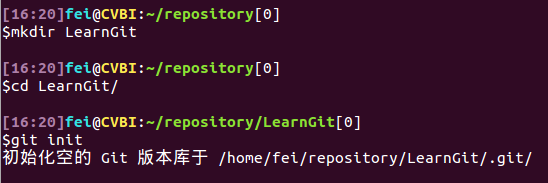
\includegraphics[width=5cm]{repository.png}}
  \end{figure}
  \end{enumerate}
\end{frame}

\subsection{Github}

\begin{frame}
  \frametitle{Github}
  \zhushadow{Github} Github是一个共享虚拟主机服务,用于存放使用Git版本控制的软件代码和内容项目。
\end{frame}


\begin{frame}
  \begin{tcolorbox}[colback=blue!15,colframe=blue!75!black]  
  My box with my title.    My box with my title.    My box with my title.  
  \end{tcolorbox}
\end{frame}

\subsection{My Project}

\begin{frame}
  \frametitle{My Project}
  
\end{frame}

\subsection{分支管理}

\begin{frame}
  \frametitle{创建与合并分支}
  \begin{center}
  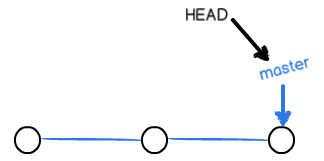
\includegraphics[width=0.2\linewidth]{1.png}
  \hspace{0.5em}
  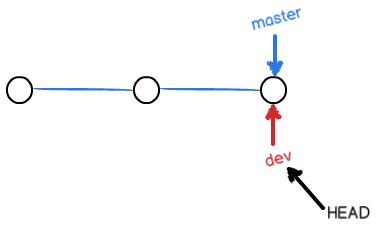
\includegraphics[width=0.2\linewidth]{2.png}
  \hspace{0.5em}
  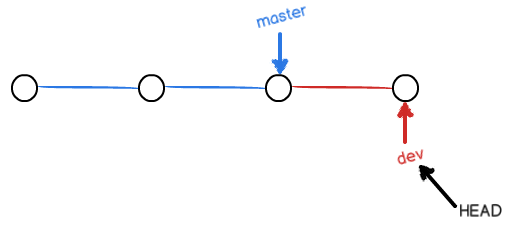
\includegraphics[width=0.2\linewidth]{3.png}
  \hspace{0.5em}
  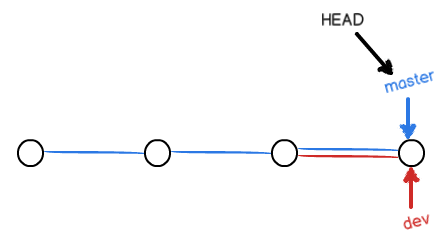
\includegraphics[width=0.2\linewidth]{4.png}
  \end{center}
  \begin{figure}[h]
  \centering
  \centerline{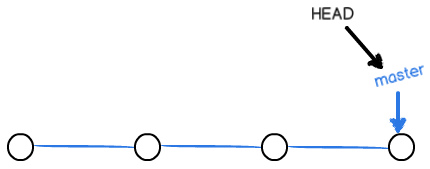
\includegraphics[width=5cm]{5.png}}
  \end{figure}
\end{frame}


\begin{frame}
  \frametitle{创建与合并分支}
  \begin{itemize}
  \item 查看分支:git branch
  \item 创建分支:git branch name
  \item 切换分支:git checkout name
  \item 创建+切换分支:git checkout -b name
  \item 合并某分支到当前分支:git merge name
  \item 删除分支:git branch -d name
  \end{itemize}
\end{frame}


\end{document}
